\documentclass[12pt]{beamer}

\hypersetup{colorlinks=true,linkcolor=red}
\usetheme{default}
\usecolortheme{albatross}

\usepackage[utf8]{inputenc}
\usepackage[russian,english]{babel}
\usepackage[T2A]{fontenc}
\usepackage{hyperref}
\usepackage[final]{listings}
\usepackage{breakurl}
\usepackage{cite}
\usepackage{perpage}

\graphicspath{{img/}}

\def\Url\Breaks{\do\/\do-}
\lstset{
  frame=single,
  breaklines=true,
  basicstyle=\tiny,
  postbreak=\raisebox{0ex}{\ensuremath{\hookrightarrow\space}},
  numbers=left
}

\lstdefinestyle{base}{
  frame=single,
  breaklines=true,
  basicstyle=\tiny,
  postbreak=\raisebox{0ex}{\ensuremath{\hookrightarrow\space}},
  moredelim=[is][\color{red}]{@}{@},
  numbers=left
}

\MakePerPage{footnote}

\title{Operating Systems}
\subtitle{Permanent Storage}
\author{Me}
\date{\today}

\begin{document}
  \begin{frame}
    \titlepage
  \end{frame}

  \begin{frame}
\frametitle{Блочные устройства}
\begin{itemize}
  \item Блочные устройства - устройсва с поблочным доступом
  \begin{itemize}
    \item общение с устройством идет порциями кратными некоторому фиксированному
    размеру - сектору
    \item типичный размер сектора - 512 байт;
    \item внутри устройство может работать с блоками произвольного размера, но
    интерфейс зачастую в 512 байтных блоках.
  \end{itemize}
  \item Типичные примеры блочных устройств:
  \begin{itemize}
    \item жесткие диски (HDD) и твердотельные накопители (SSD);
    \item оптические диски (CD, DVD, etc);
    \item даже USB Flash накопители...
  \end{itemize}
\end{itemize}
\end{frame}

  \begin{frame}
\frametitle{Механические диски (HDD)}
\begin{columns}
  \begin{column}{.6\linewidth}
    \begin{center}
      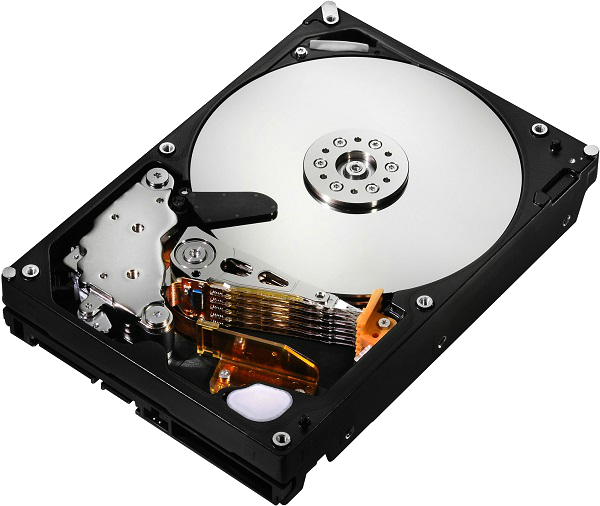
\includegraphics[width=.9\linewidth]{hdd.png}
    \end{center}
  \end{column}
  \begin{column}{.55\linewidth}
    Три основных части:
    \begin{itemize}
      \item вращающиеся диски (platters);
      \item подвижная рука (arm);
      \item читающие/пишушие головы (heads);
    \end{itemize}
  \end{column}
\end{columns}
\end{frame}

\begin{frame}
\frametitle{Скорость HDD}
\begin{itemize}
  \item Скорость вращения дисков HDD:
  \begin{itemize}
    \item при скорости 7200 оборотов в минуту - один оборот 8-9 мс;
    \item чтобы записать/прочитать данные нужно поставить голову над/под нужным
    цилиндром и подождать, пока нужное место диска "доедет" до головы.
  \end{itemize}
  \item Скорость позиционирования читающей/пишушей головы:
  \begin{itemize}
    \item время определяется опять же миллисекундами.
  \end{itemize}
  \item Скорость работы диска доминируется поиском:
  \begin{itemize}
    \item скорость вращения диска + позиционирование головы;
    \item random IO гораздо медленнее sequential IO.
  \end{itemize}
\end{itemize}
\end{frame}

\begin{frame}
\frametitle{Скорость HDD}
\begin{center}
  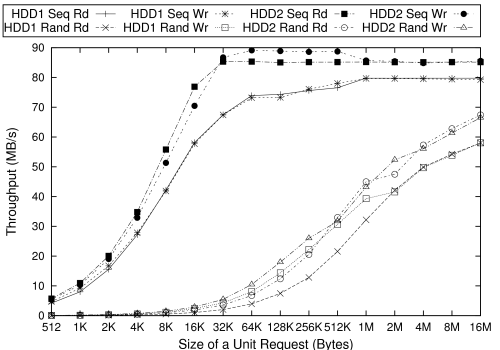
\includegraphics[width=.8\linewidth]{hdd_perf.png}
\end{center}
\end{frame}

  \begin{frame}
\frametitle{Твердотельные накопители (SSD)}
\end{frame}

  \begin{frame}
\frametitle{Интерфейс для работы с дисками}
\begin{itemize}
  \item Современные диски содержат встроенные контроллеры:
  \begin{itemize}
    \item т. е. вам не нужно заботиться о физической организации диска (на каком
    диске, в каком цилинде, в каком секторе хранится блок данных и тд.);
    \item вам нужно сформировать корректную команду и передать ее диску.
  \end{itemize}
  \item Есть два более или менее распространенных набора команд:
  \begin{itemize}
    \item ATA - получил популярность благодаря использованию в PC;
    \item SCSI - используется в производительных системах хранения.
  \end{itemize}
\end{itemize}
\end{frame}

  \begin{frame}
\frametitle{Планирование потоков}
\begin{itemize}
  \item Мы знаем что-такое потоки и как между ними переключаться
  \begin{itemize}
    \item осталось разобраться с мелочами - когда и на какой конкретно поток
    переключаться.
  \end{itemize}
  \item Начнем с простой и нереалистичной задачи:
  \begin{itemize}
    \item мы заранее знаем все задачи, которые нужно выполнить;
    \item и про каждую задачу знаем сколько времени потребуется на выполнение;
    \item более того мы выполняем каждую задачу от начала до конца без
    переключений, т. е. нужно только определить порядок выполнения задач.
  \end{itemize}
\end{itemize}
\end{frame}

\begin{frame}
\frametitle{SJF 1/2}
\begin{columns}
  \begin{column}{0.5\linewidth}
    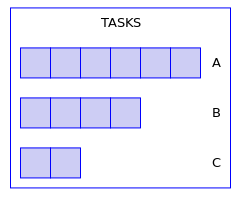
\includegraphics[width=0.9\linewidth]{sjf_tasks.png}
  \end{column}
  \begin{column}{0.5\linewidth}
    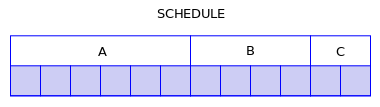
\includegraphics[width=0.9\linewidth]{sjf_schedule0.png}
    \begin{itemize}
      \item 3 задачи, по 6, 4 и 2 единиц;
      \item суммарно 12 единиц времени;
      \item среднее время ожидания заверешения:
      ${{6+10+12}\over{3}}=9.\left(3\right)$
    \end{itemize}
  \end{column}
\end{columns}
\end{frame}

\begin{frame}
\frametitle{SJF 2/2}
\begin{columns}
  \begin{column}{0.5\linewidth}
    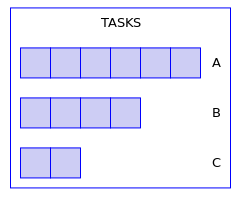
\includegraphics[width=0.9\linewidth]{sjf_tasks.png}
  \end{column}
  \begin{column}{0.5\linewidth}
    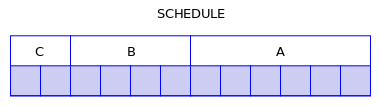
\includegraphics[width=0.9\linewidth]{sjf_schedule1.png}
    \begin{itemize}
      \item теже 3 задачи, по 6, 4 и 2 единиц;
      \item суммарно 12 единиц времени (о чудо!);
      \item среднее время ожидания заверешения:
      ${{2+6+12}\over{3}}=6.\left(6\right)$
    \end{itemize}
  \end{column}
\end{columns}
\end{frame}

\begin{frame}
\frametitle{Shortest Job First}
\begin{itemize}
  \item Упорядочив задачи по времени исполнения от меньшей к большей получим
  оптимальное по среднему времени ожидания расписание
  \begin{itemize}
    \item отсюда и Shortest Job First (SJF).
  \end{itemize}
\end{itemize}
\end{frame}

\begin{frame}
\frametitle{Блокировка потока}
\begin{itemize}
  \item Потоки могут быть заблокированы:
  \begin{itemize}
    \item поток может ожидать ввода от пользователя - даже самый быстрый
    пользователь очень медленный по сравнению с CPU;
    \item поток может ожидать получения данных по сети;
    \item поток может запросить доступ к медленному устройству и ждать
    прерывания от него (например, диск);
    \item другими словами поток может быть заблокирован в ожидании завершения
    операции ввода/вывода.
  \end{itemize}
  \item Заблокированным потокам нет смысла отдавать CPU:
  \begin{itemize}
    \item все что они могут делать, так это ждать завершения IO.
  \end{itemize}
\end{itemize}
\end{frame}

\begin{frame}
\frametitle{Динамическое создание и завершение}
\begin{itemize}
  \item Потоки создаются и завершаются динамически:
  \begin{itemize}
    \item новый поток может быть создан в любой момент;
    \item т. е. все потоки заранее не известны;
    \item существующий поток может завершиться;
    \item т. е. мы не знаем время необходимое потоку для завершения.
  \end{itemize}
\end{itemize}
\end{frame}

\begin{frame}
\frametitle{Round Robin}
\begin{itemize}
  \item Самый простой вариант планирования в реалистичных условиях - отдавать
  процессор активным потокам по очереди:
  \begin{itemize}
    \item все задачи ожидающие CPU организованы в очередь;
    \item каждой задаче выделяется квант времени;
    \item задача снимается с CPU по истечении кванта;
    \item задача может отдать CPU самостоятельно перед истечением кванта;
    \item незавершившаяся задача снятая с CPU возвращается в конец очереди.
  \end{itemize}
\end{itemize}
\end{frame}

\begin{frame}
\frametitle{Round Robin, pros}
\begin{itemize}
  \item Round Robin - является простым реалистичным алгоритмом планирования:
  \begin{itemize}
    \item выбор следующего потока требует $O\left(1\right)$;
    \item зная ограничение на количество потоков, мы можем ограничить
    максимальное время ожидания.
  \end{itemize}
  \item Гарантия, когда время реакции системы на событие (прерывание) жестко
  ограничено сверху - гарантия жесткого реального времени:
  \begin{itemize}
    \item т. е. Real Time на самом деле - это не про скорость;
    \item Round Robin сам по себе не нарушает гарантию реального времени.
  \end{itemize}
\end{itemize}
\end{frame}

\begin{frame}
\frametitle{Round Robin, cons 1/3}
\begin{itemize}
  \item IO Bounded поток - поток, работа которого ограничена скоростью IO:
  \begin{itemize}
    \item такие потоки часто не вырабатывают свой квант полностью, а отдают
    CPU раньше заблокировавшись на IO;
    \item типичный пример: текстовый редактор.
  \end{itemize}
  \item CPU Bounded поток - работа потока ограничивается скоростью CPU:
  \begin{itemize}
    \item такие потоки редко не вырабатывают свой квант полностью, они всегда
    хотят получить CPU в свое пользование;
    \item типичные примеры: численные расчеты, задачи рендеринга.
  \end{itemize}
\end{itemize}
\end{frame}

\begin{frame}
\frametitle{Round Robin, cons 2/3}
\begin{center}
  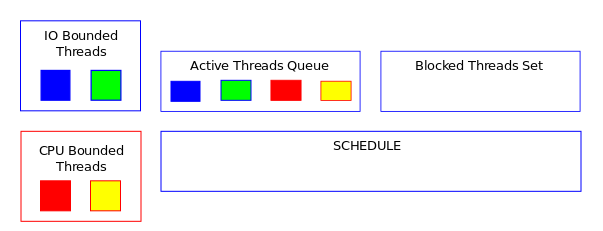
\includegraphics[width=0.8\linewidth]{rr0.png}
\end{center}
\begin{center}
  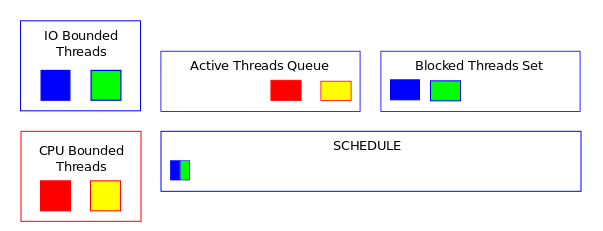
\includegraphics[width=0.8\linewidth]{rr1.png}
\end{center}
\end{frame}

\begin{frame}
\frametitle{Round Robin, cons 2/3}
\begin{center}
  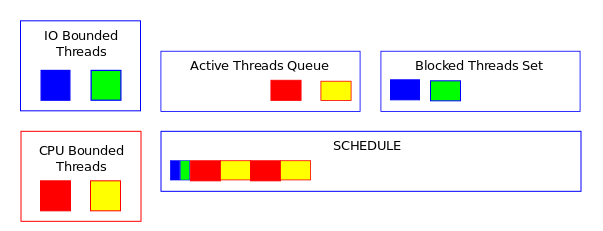
\includegraphics[width=0.8\linewidth]{rr2.png}
\end{center}
\begin{center}
  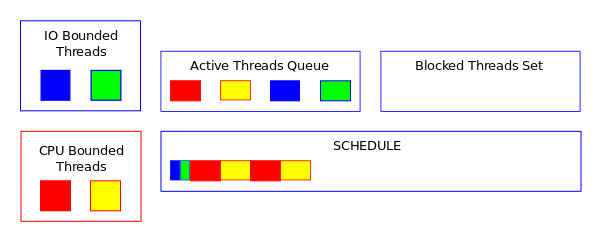
\includegraphics[width=0.8\linewidth]{rr3.png}
\end{center}
\end{frame}

\begin{frame}
\frametitle{Round Robin, cons 3/3}
\begin{center}
  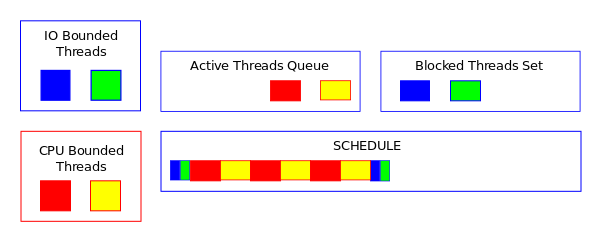
\includegraphics[width=0.8\linewidth]{rr4.png}
\end{center}
\begin{center}
  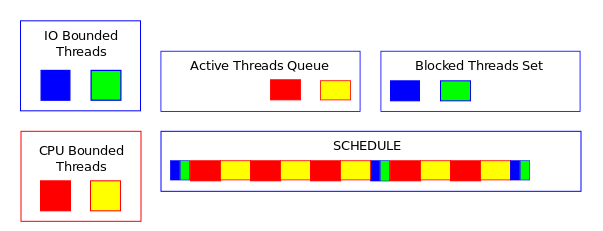
\includegraphics[width=0.8\linewidth]{rr5.png}
\end{center}
\end{frame}

\begin{frame}
\frametitle{Честность Round Robin}
\begin{itemize}
  \item IO Bounded задачи при Round Robin получают меньше CPU:
  \begin{itemize}
    \item они не вырабатывают свой квант и блокируются - не выработанное время
    никак не компенсируется.
  \end{itemize}
  \item IO Bounded задачи часто являются интерактивными, т. е. работают с
  пользователем, а пользователь не любит ждать
  \begin{itemize}
    \item однако когда поток разблокируется он встает в конец очереди и ждет
    пока вся очередь отработает.
  \end{itemize}
  \item Итого IO Bounded задачи получают меньше CPU, а задержка по доступу к CPU
  у них такая же как и у всех
  \begin{itemize}
    \item не все задачи одинаковые, и может потребоваться разделение задач на
    классы и приоритизация.
  \end{itemize}
\end{itemize}
\end{frame}

\begin{frame}
\frametitle{Completely Fair Scheduler 1/2}
\begin{itemize}
  \item Планировщик по-умолчанию в Linux Kernel
  \begin{itemize}
    \item пытается гарантировать идеальную честность отслеживая "виртуальное"
    отработанное время каждого потока;
    \item поток с нименьшим "виртуальным" временем получает CPU;
    \item выбор следующего потока требует $O\left(log n\right)$.
  \end{itemize}
\end{itemize}
\end{frame}

\begin{frame}
\frametitle{Completely Fair Scheduler 2/2}
\begin{itemize}
  \item Как обрабатывать разблокированные потоки вновь созданные потоки?
  \begin{itemize}
    \item нельзя просто верунть разблокированные задачи в очередь, т. к. их
    "виртуальное" время может сильно отстать от других и они станут "слишком
    приоритетными";
    \item для очереди потоков поддерживается "минимальное виртуальное" время,
    для новых и разблокированных задач проверяется, что их "виртуальное" время
    не сильно отстает от "минимального виртуального" времени.
  \end{itemize}
\end{itemize}
\end{frame}

\begin{frame}
\frametitle{Лотерейное планирование 1/2}
\begin{itemize}
  \item Самый "простой" способ обеспечить честность - рандомизация:
  \begin{itemize}
    \item выдадим каждому потоку набор лотерейных билетов;
    \item вероятность получения CPU в каждом "розыгыше" определяется количеством
    билетов у потока.
  \end{itemize}
  \item Статические и динамические приоритеты:
  \begin{itemize}
    \item потокам можно выдавать разное количество билетов согласно приоритету;
    \item кроме того, потоки могут временно передавать билеты друг другу и
    изменять свои приоритеты;
    \item например, поток \emph{A} пытается получить доступ к ресурсу \emph{X},
    но ресурс \emph{X} уже занят потоком \emph{B} - пусть \emph{A} передаст свои
    билеты \emph{B}, чтобы он раньше закончил работу с \emph{X}.
  \end{itemize}
\end{itemize}
\end{frame}

\begin{frame}
\frametitle{Лотерейное планирование 2/2}
\begin{itemize}
  \item При честной рандомизации возможны выбросы
  \begin{itemize}
    \item рандомизация гарантирует математическое ожидание времени CPU, но
    возможны отклонения от математического ожидания;
    \item чтобы ограничить отклонения, мы можем "удалять" выигравший билет;
    \item когда все билеты были "удалены", мы раздаем билеты заново;
    \item выбросы все еще возможны, но они ограничены (почти).
  \end{itemize}
\end{itemize}
\end{frame}

  \begin{frame}
\frametitle{Скорость CPU, памяти и дисков}
\begin{itemize}
  \item Некоторое время назад (80-90-ые года) скорость CPU росла довольно быстро
  \begin{itemize}
    \item вместе со скоростью CPU росли объемы оперативной памяти и дисков.
  \end{itemize}
  \item Однако скорость оперативной памяти и дисков не успевала за ростом:
  \begin{itemize}
    \item разрыв между скоростью памяти и CPU так или иначе заполняется кешами;
    \item но между оперативной памятью и дисками просто пропасть.
  \end{itemize}
\end{itemize}
\end{frame}

\begin{frame}
\frametitle{Массивы независимых (недорогих) дисков}
\begin{itemize}
  \item RAID (Redundant Array of Independent (Inexpenisve) Disks) - объединение
  из нескольких физических устройств в одно логические устройство:
  \begin{itemize}
    \item несколько дисков позволяют достигать большего объема;
    \item при дублировании данных на несколько дисков мы можем читать данные с
    любого из них - несколько параллельных запросов повышают производительность;
    \item имея копии данных мы можем переживать поломки дисков/порчу данных.
  \end{itemize}
\end{itemize}
\end{frame}

\begin{frame}
\frametitle{Redundancy is important}
\begin{itemize}
  \item В спецификации дисков зачастую указывают параметры MTTF/MBTF/AFR:
  \begin{itemize}
    \item MTTF (Mean Time to Failure) - для SSD где-то в районе 2 млн. часов;
    \item для массива из 1000 одинаковых дисков получим что-то вроде 2000
    часов;
    \item чем больше независмых устройств - тем больше вроятность отказа
    системы.
  \end{itemize}
  \item Для массива из дисков полезен еще дополнительный параметр MTTR:
  \begin{itemize}
    \item MTTR (Mean Time To Repair) - время необходимое на обнаружения сбоя
    диска, его замену и восстановление данных на нем;
    \item никакой RAID вас не спасет, если вам нужно 100500 лет чтобы заменить
    плохой диск.
  \end{itemize}
\end{itemize}
\end{frame}

\begin{frame}
\frametitle{RAID}
\framesubtitle{Mirroring}
\begin{itemize}
  \item Самый очевидный способ повысить надежность - простое дублирование:
  \begin{itemize}
    \item вы просто пишите каждую порцию данных на 2 (N) дисков параллельно;
    \item при таком подходе можно переживать 1 (N-1) отказ диска.
  \end{itemize}
  \item Минусы:
  \begin{itemize}
    \item требуется в 2 (N) раза больше пространства;
    \item "хвосты" - запись со скоростью самого медленного диска.
  \end{itemize}
  \item Плюсы:
  \begin{itemize}
    \item чтение в 2 (N) раза быстрее - любая порция данных может быть прочитана
    с любого из дисков (если он в строю);
    \item т. е. мы можем обрабатывать несколько запросов на чтение параллельно.
  \end{itemize}
\end{itemize}
\end{frame}

\begin{frame}
\frametitle{RAID}
\framesubtitle{Parity}
\begin{center}
  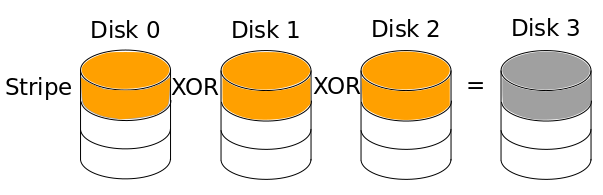
\includegraphics[width=.8\linewidth]{parity.png}
\end{center}
\begin{itemize}
  \item Вместо полного дублирования мы можем использовать проверку четности:
  \begin{itemize}
    \item пусть у нас будет N дисков с данными - на каждый из них пишется своя
    порция информации;
    \item добавим к ним еще один диск - диск четности;
    \item диск четности хранит XOR соответствующих бит дисков с данными;
  \end{itemize}
\end{itemize}
\end{frame}

\begin{frame}
\frametitle{RAID 2}
\framesubtitle{Matrix Form}
\[
  \left(
    \begin{array}{cccc}
      1 & 1 & 1 & 1
    \end{array}
  \right) \times \left(
    \begin{array}{c}
      d_0 \\
      d_1 \\
      d_2 \\
      d_3
    \end{array}
  \right) = 0
\]
\begin{itemize}
  \item Мы можем записать условие четности в матричном виде:
  \begin{itemize}
    \item сложение - XOR;
    \item умножение - AND;
    \item т. е. XOR всех бит данных с битом четности должен давать 0.
  \end{itemize}
\end{itemize}
\end{frame}

\begin{frame}
\frametitle{RAID}
\framesubtitle{Generalized Parity}
\[
  \left(
    \begin{array}{ccccccc}
      1 & 0 & 1 & 0 & 1 & 0 & 1 \\
      0 & 1 & 1 & 0 & 0 & 1 & 1 \\
      0 & 0 & 0 & 1 & 1 & 1 & 1
    \end{array}
  \right) \times \left(
    \begin{array}{c}
      d_0 \\
      d_1 \\
      d_2 \\
      d_3 \\
      d_4 \\
      d_5 \\
      d_6
    \end{array}
  \right) = \left(
    \begin{array}{c}
      0 \\
      0 \\
      0
    \end{array}
  \right)
\]
\begin{itemize}
  \item Мы можем проверять четность для некоторого подмножества бит
  \begin{itemize}
    \item если каждый диск входит хотя бы в одно подмножество;
    \item и для каждой пары дисков есть подмножество, в которое входит только
    один из них;
    \item то мы легко можем исправлять сразу две ошибки.
  \end{itemize}
\end{itemize}
\end{frame}

\begin{frame}
\frametitle{RAID}
\begin{itemize}
  \item В общем случае нужную систему уравнений нам дают коды Хэмминга:
  \begin{itemize}
    \item для $C$ дисков с битами четности можно использовать до $2^C - 1 - C$
    дисков с данными;
    \item т. е. всего $2^C - 1$ дисков;
    \item и переживать потерю любых двух дисков.
  \end{itemize}
  \item Недостатки:
  \begin{itemize}
    \item нужно сравнительно много дисков, чтобы получить какой-то выигрыш по
    сравнению с Mirroring нужно как минимум 7 дисков;
    \item запись происходит со скоростью самого медленного диска.
  \end{itemize}
  \item Достоинства:
  \begin{itemize}
    \item дополнительные расходы дискового пространства уменьшаются
    экспоненциально.
  \end{itemize}
\end{itemize}
\end{frame}

\begin{frame}
\frametitle{Финальные замечания про RAID-ы}
\begin{itemize}
  \item Мы предполагали, что диски могут выходить из строя целиком
  \begin{itemize}
    \item если диск вышел из строя целиком, то это легко обнаржить, т. е. мы
    всегда знаем где ошибка;
    \item что если диск все еще работает, но некоторые данные на нем
    испортились?
    \item добавим к каждой порции данных на диске контрольную сумму (хеш).
  \end{itemize}
\end{itemize}
\end{frame}

\begin{frame}
\frametitle{Финальные замечания про RAID-ы}
\begin{itemize}
  \item Мы рассмотрели возможность исправления 1 или 2 ошибок, при условии, что
  мы знаем где эти ошибки произошли
  \begin{itemize}
    \item в общем случае можно построить код позволяющий исправить любое
    количество ошибок;
    \item например, коды Боуза-Чоудхури-Хоквингема в общем и коды Рида-Соломона
    как частный случай.
  \end{itemize}
\end{itemize}
\end{frame}


  \begin{frame}
  \begin{center}
  \Huge Q\&A
  \end{center}
  \end{frame}
\end{document}
